\documentclass[dvipdfmx]{jsarticle}
\usepackage[dvipdfmx]{graphicx}
\usepackage{amsmath, amssymb}
\usepackage{mathtools}
\usepackage{here}
\renewcommand{\thefigure}{\thesection.\arabic{figure}}
\setcounter{section}{3}
\setcounter{figure}{5}

\begin{document}

\section*{3.2.1 後半}
一様散乱下での受信信号$r(t)$のPSD(パワースペクトル密度)を求めるには,$A_{r_I, r_Q}(\tau) = 0$として(3.23),(3.28),フーリエ関数の簡単な性質を用いて,次のようになる.

\begin{equation}
S_{rI}(f) = \mathcal{F} [A_{rI}(\tau)] = .25[S_{rI}(f - f_c) + S_{rI}(f + f_c)] =
\begin{dcases}
\frac{P_r}{4 \pi f_D} \frac{1}{\sqrt{1 - (\frac{|f - f_c|}{f_D})^2}} & |f - f_c| \leqq f_D \\
0 & \mathrm{else}
\end{dcases}
\tag{3.29}
\end{equation}

\noindent
なお,このPSDは積分して全受信電力$P_r$となる.

PSDは,マルチパス成分に関連する電力密度をそのドップラー周波数の関数としてモデル化しているので,マルチパスに関連するドップラーによるランダム周波数の分布(pdf)と見ることができる.
図3.6から,PSD $S_ri(f)$は$f = \pm f_D$で無限大となり,その結果,PSD $S_r(f)$は $f = \pm f_c \pm f_D$で無限大となることが分かる.
一様散乱モデルは近似に過ぎないので,実際にはこのようにはならないが,散乱体が密集している環境では,一般に最大ドップラー周波数に近い周波数でPSDが最大になる.
この振る舞いの直観的理解は,コサイン関数の性質と,我々の仮定において,PSDがランダムドップラー周波数$f_D(\theta)$のpdfに対応する事実から来るものである.
これを理解するには,均一散乱の仮定が同じ平均パワーで全ての角度から一様に到着する多くの散乱経路に基づいていることに注意しなければならない.
したがって,ランダムに選択されたパスの$\theta$は,$[0, 2\pi]$上の一様な確率変数とみなすことができる.
そして,ランダムドップラー周波数$f(\theta)$の分布$p_{f_\theta}(f)$は$\theta$の分布から得ることができる.
定義によれば,$p_{f_\theta}(f)$はドップラー周波数$f$における散乱体の密度に比例する.
したがって,$S_{rI}(f)$もこの密度に比例し,pdf $p_{f_\theta}$から$\theta$を特徴づけることができる.
この特徴づけのために,図3.7では$f_D(\theta) = f_D \cos (\theta) = v / \lambda \cos (\theta)$と,$\underline{f}_D(\theta)$に対する点線の直線セグメント近似値$f_D (\theta)$をプロットしている.
この図の右側には,PSD $S_{ri}(f)$を,ドップラー近似$\underline{f}_D (\theta)$に対応する点線の直線セグメント近似値$\underline{S}_{ri}(f)$と共にプロットしている.
相対的に広い$\theta$の範囲で,$\cos (\theta) \approx \pm 1$となることが分かる.
したがって,この範囲の値の到来角を持つマルチパス成分は,ドップラー周波数$f_D(\theta) \approx \pm f_D$となり,これらのマルチパス成分全てに関連する電力は$f \approx f_D$のPSDにおいて加算されることとなる.
このことは,我々の近似では,図左の$\underline{f}_D(\theta) = \pm f_D$の区間が,図右のpdf近似$\underline{S}_{r_i} (f)$の$\pm f_D$におけるデルタ関数を導いたということによって示されている.
図左側の$\underline{f}_D(\theta)$が一様な傾きを持つ区間は,各角度の増分においてパワーを寄与するマルチパス成分が1つであるため,図右側の$\underline{S}_{ri}(f)$の平坦部を導出している.
より典型的なマイクロセルと室内環境に対応する非一様散乱における自己相関とPSDの公式は,[5, Chapter 1],  [11, Chapter 2]に記載されている.

\begin{figure}[H]
\begin{center}
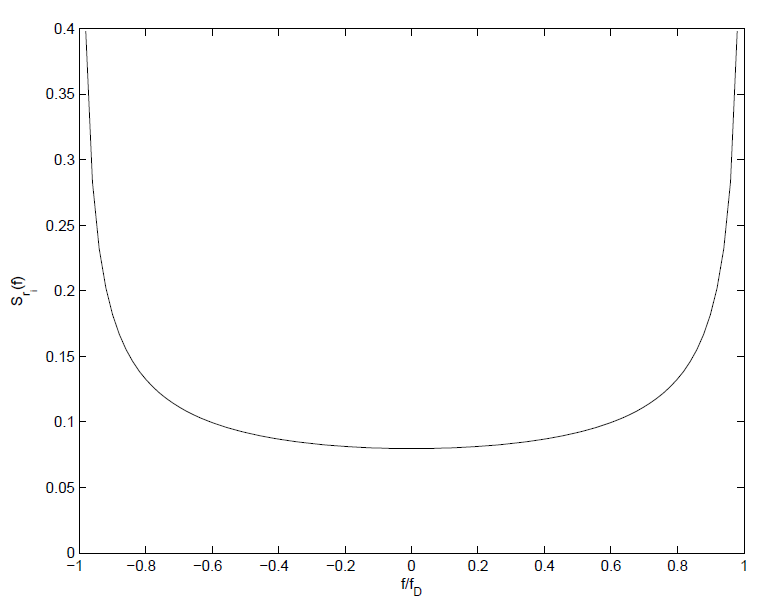
\includegraphics[width=0.6\linewidth]{"./spring_lec/psd1.png"}
\end{center}
\caption{同相,直角位相のパワースペクトル密度}
\end{figure}

\begin{figure}[htbp]
\begin{center}
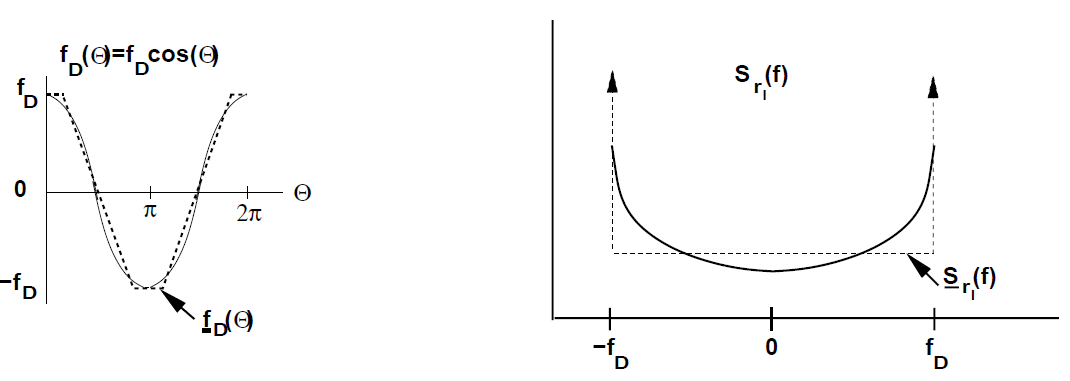
\includegraphics[width=0.85\linewidth]{"./spring_lec/psd2.png"}
\end{center}
\caption{コサインと直線部分によるPSDの近似値}
\end{figure}

PSDはフェージングプロセスのシミュレーションを構築する際に有用である.
狭帯域フェージング過程の包絡線をシミュレーションするための一般的な方法は,PSD $N_0 / 2$を持つ2つの独立した白色ガウス雑音源を,次の式を満たす,周波数応答$H(f)$のローパスフィルタに通すことである.

\begin{equation}\label{}
S_{r_I}(f) = S_{r_Q}(f) = \frac{N_0}{2} |H(f)|^2
\tag{3.30}
\end{equation}

\noindent
フィルタ出力は,PSDs $S_{r_I}(f)$,$S_{r_Q}(f)$による狭帯域フェージングプロセスの同相成分と直交成分に相当する.離散フィルタを用いた同様の手順で,離散フェージングプロセスを生成することができる.

ほとんどの通信シミュレーションパッケージ(例:Matlab,COSSAP)には,この方法に基づいて狭帯域フェージングをシミュレーションするモジュールが標準的に備わっている.このシミュレーション方法の詳細,および代替の方法は,[11, 6, 7]に記載されている.
これで,狭帯域無線通信路で示される電力対距離の3つの特性に関するモデルが完成した.これらの特性は,第2章で発展させた経路損失とシャドウィングのモデルに,狭帯域フェージングを加えた図3.8に示されている.
この図では,パスロス指数$\gamma$とともにパスロスが$d^{\gamma}$にしたがって減少することによる信号パワーの減少,非相関距離$X_c$のオーダーで変化するシャドウィングによるより急速な変動,および信号波長のオーダーで変化するマルチパスフェージングによる非常に急速な変動が見られる.
パスロスとシャドウィングが一定である距離で,この図の小さな区間を拡大すると,図3.9が得られる.ここで,受信電力対直線距離$d = vt$ (対数距離ではない) におけるdB変動を示す.この図では,平均受信電力$P_r$は0 dBmに正規化されている.
一定の速度 $v$ で移動する受信機では,この図に示されるような受信電力の時間的な変動が発生する.

\begin{figure}[htbp]
\begin{center}
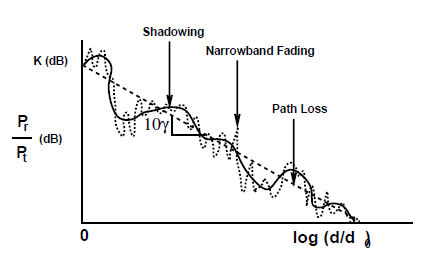
\includegraphics[width=0.7\linewidth]{"./spring_lec/fading1.png"}
\end{center}
\caption{パスロス,シャドウィング,狭帯域フェージングの複合}
\end{figure}

\begin{figure}[htbp]
\begin{center}
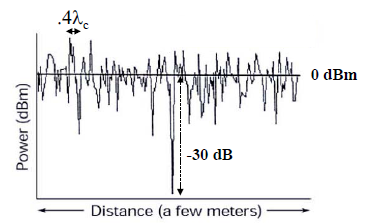
\includegraphics[width=0.7\linewidth]{"./spring_lec/fading2.png"}
\end{center}
\caption{狭帯域フェージング}
\end{figure}

\end{document}